%---------------------------------------------------------------------------%
%->> Frontmatter
%---------------------------------------------------------------------------%
%-
%-> 生成封面
%-
\maketitle% 生成中文封面
\MAKETITLE% 生成英文封面
%-
%-> 作者声明
%-
\makedeclaration% 生成声明页
%-
%-> 中文摘要
%-
\intobmk\chapter*{摘\quad 要}% 显示在书签但不显示在目录
\setcounter{page}{1}% 开始页码
\pagenumbering{Roman}% 页码符号

目标跟踪是计算机视觉领域中最重要和最具挑战性的研究课题之一,在智能监控、自动驾驶等领域有着潜在广阔的应用前景。目标跟踪的核心是估计图像序列的每帧中目标的运动状态。目标跟踪是计算机视觉领域的中层部分,为目标的行为理解提供了基础,因此具有非常重要的理论研究价值。同时,它具有广泛的实际应用,包括视频监控,交通流量监控,视频压缩和人机交互等。例如,目标跟踪已成功应用于监控居民区,停车场和银行中的人类活动(例如W4系统[1]和VSAM项目[2])。在交通运输领域,目标跟踪也被广泛用于交通流量监控[3],行人计数[4]等任务。
由于目标跟踪的理论价值与应用价值,众多科研机构和公司都投入到这项研究中。然而,目标跟踪领域存在很多理论和技术问题有待解决,如运动模糊、光照变化、非刚性目标的形变、视角的变化导致的目标旋转、遮挡等。近年来深度学习的突破为解决目标跟踪中的一系列问题带来了可能。
深度学习是基于人工神经网络的机器学习方法。在过去的十年中,深度学习技术得到了飞速发展,已成功应用于计算机视觉,语音识别,自然语言处理,音频识别,社交网络过滤,机器翻译,生物信息学,药物设计等领域。如何利用深度学习方法,尤其是深度卷积神经网络解决跟踪过程中遇到的复杂问题,具有较大的研究价值和研究空间。

本文利用卷积神经网络强大的表征能力,为视频目标跟踪算法的特征表示,表观模型建模,运动模型建模,模型更新等方面进行了改进,有效提高的算法的性能。主要的工作和贡献有:

\begin{figure}
\centering
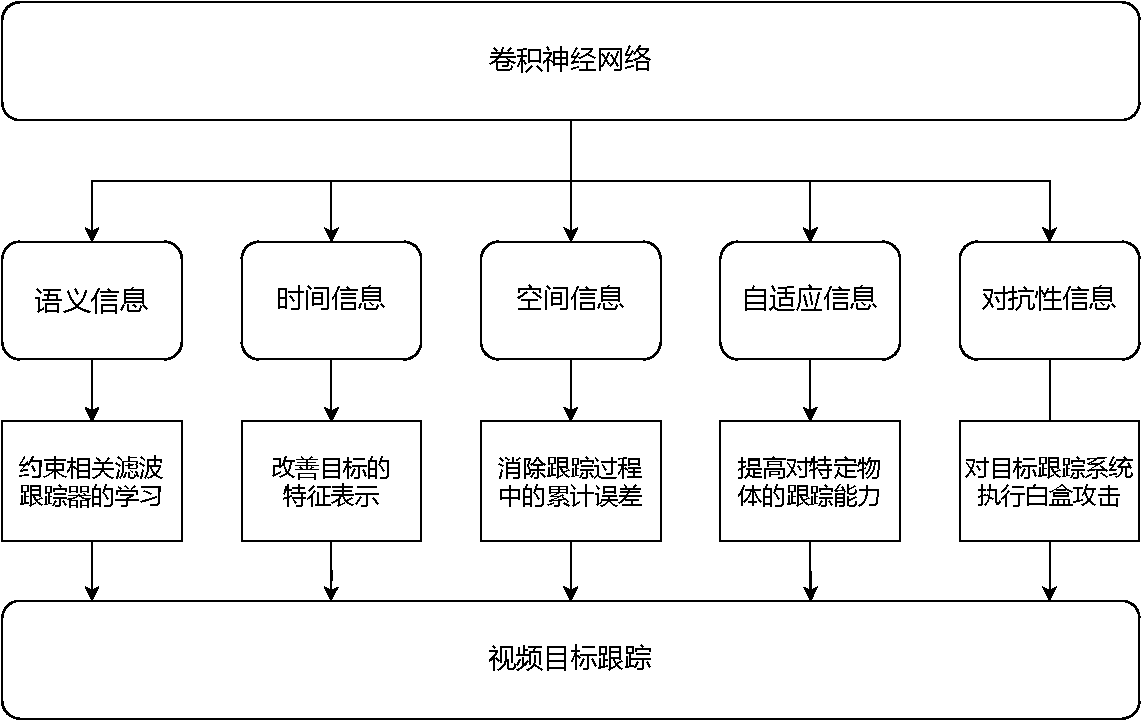
\includegraphics[width=0.75\textwidth]{Img/paper_arch.pdf}
\caption{文章组织架构}
\end{figure}

\begin{itemize}
\item{\textbf{提出了一种语义信息引导的视频目标跟踪算法。}我们利用卷积神经网络获得目标的\textbf{语义信息}用于约束跟踪器的训练过程,从而提高跟踪的效果。具体而言,首先:我们提出了实例引导的相关滤波器。利用神经网络学习图像的实例级别的语义分割模板约束相关滤波器的学习。其次,针对离线训练的语义分割结果和在线学习的相关滤波结果具有互补性这一特点,我们提出了跟踪结果的自纠正机制,利用分割结果纠正相关滤波结果。我们在多个具有挑战性的视频目标跟踪数据库上验证了这些创新点在视频目标跟踪应用中的有效性。}
\item{\textbf{提出了一种空间信息增强的视频目标跟踪算法。}不同于前人工作中,在空间上是局部搜索的,以确定目标位置,我们引入了更丰富的\textbf{空间信息}。具体而言,该跟踪算法在运动模型方面进行优化,始终在整个图像平面内感知物体的位置信息,弥补传统的局部搜索机制中目标搜索范围有限的缺点,从而能够有效地减少累积误差并提高鲁棒性。为了进一步减轻近似物体的干扰,我们提出了一个端到端训练的轨迹预测模块,能够利用物体的历史轨迹信息和当前帧的表观信息预测物体在当前帧的每个空间位置上出现的可能性。我们在多个视频跟踪标准评测库上验证了这些创新点的有效性,并大幅度提高了跟踪算法的准确性和鲁棒性。}
\item{\textbf{提出了时间信息增强的视频目标跟踪算法。}该算法主要在特征提取方面对基于孪生网络的视频目标跟踪算法进行优化。首先,我们从基于孪生网络的在线视频跟踪算法鲁棒性不足问题出发,将\textbf{时间信息}引入在线视频目标跟踪中。通过来自相邻帧的目标表观信息的聚合,使得目标表观特征更加丰富,弥补基于孪生网络的视频目标跟踪算法局限于从单帧提取目标表观,从而对目标表观表示能力不足的缺点,从而提高跟踪的效果,实现鲁棒的跟踪。在端到端时间聚合的基础上,我们通过引入对抗性 dropout 模块,并通过在大规模数据集上端到端训练,使得孪生网络跟踪器在目标由于运动模糊等导致的表观不佳的情况下具有更好的表现,从而进一步提高跟踪的鲁棒性。我们在目前流行的视频目标跟踪评测库上进行了算法的对比试验以及成分分析实验,从而验证算法改进的有效性。}
\item{\textbf{提出了自适应信息增强的视频目标跟踪算法}该算法主要在模型自适应方面对基于孪生网络的视频目标跟踪算法进行优化。我们引入了\textbf{自适应信息}。前人工作:离线训练。目的:提高了算法对特定物体的自适应能力。首先,通过对模板图像的像素进行微小的扰动,从而改善孪生网络跟踪器对于特定目标的跟踪性能。该自适应性信息通过对模板图像进行梯度的反向传播计算得到,以可插拔的方式轻松添加到现有孪生网络跟踪器中,而无需修改网络模型的参数。在线跟踪时,仅在第一帧进行数次梯度传播和模板图像像素值更新,实现目标的事实跟踪。我们同样在多个视频目标跟踪评测库上验证了算法的有效性,并在精确度与实时性上取得了较好的结果。}
\item{\textbf{将对抗性信息应用于基于孪生网络的视频目标跟踪算法}我们引入了\textbf{对抗信息},提出了一种对抗攻击算法,目的:以证明现有跟踪器的鲁棒性不太行。具体来说,我们为基于孪生网络的视频目标跟踪算法生成视频无关的通用扰动,从而使得跟踪器做出错误的行为。我们为模板图像添加微小的扰动,为搜索图像添加小的补丁,这样,跟踪器预测到补丁的位置而不是目标的位置。通过离线的大规模视频目标跟踪数据集训练对抗性扰动信息,从而实现有效的攻击。我们在多个视频目标跟踪标准评测库上验证了所提出的对抗性信息的有效性,同时验证了其在不同主干网络和不同跟踪框架的可迁移性。}
\end{itemize}

基于上述方法和创新,我们的跟踪算法在多个公开数据集上都取得了当时最好或者领先的评测结果。同时,上述方法和创新,对于其他计算机视觉问题和应用,例如视频分割、视频姿态估计等,也有一定的借鉴意义。

\keywords{相关滤波,视频目标跟踪,深度学习,卷积神经网络}% 中文关键词
%-
%-> 英文摘要
%-
\intobmk\chapter*{Abstract}% 显示在书签但不显示在目录

This paper is a help documentation for the \LaTeX{} class ucasthesis, which is  a thesis template for the University of Chinese Academy of Sciences. The main content is about how to use the ucasthesis, as well as how to write thesis efficiently by using \LaTeX{}.

\KEYWORDS{University of Chinese Academy of Sciences (UCAS), Thesis, \LaTeX{} Template}% 英文关键词
%---------------------------------------------------------------------------%
